%!TEX root=../Vorlage_DA.tex
%	########################################################
% 				Projektbeschreibung
%	########################################################


%	--------------------------------------------------------
% 	Überschrift, Inhaltsverzeichnis
%	--------------------------------------------------------
\chapter{Interpreter}


%	--------------------------------------------------------
% 	Allgmeine Hinweise
%	--------------------------------------------------------
\section{Allgemeiner Teil (Theorie)}

\subsection{Aufbaumöglichkeiten eines Interpreters}

\subsubsection{Bytecode Interpreter}
Bei der Compilierung wird eine Zwischensprache erzeugt, welcher aus einer Sammlung von Befehlen besteht. Dadurch wird das System
betriebssystemunabhängig und der Code ist nahezu Hardwareunabhängig.

Jedoch muss zum Ausfürhen des Programmes, welche in die Zwischensprache übersetzt wurde, eine Virtuelle Maschine vorhanden sein.
Dadurch dass während der Laufzeit nun während der Ausfürhung des Programmes kompiliert werden muss, sinkt die Geschwindigkeit gegenüber
nativ compilierten Programmen.

Durch die Verwendung des Just-in-time compilation Verfahrens kann die Geschwindigkeit wieder verbessert werden.

\subsubsection{Abstrakter Syntax Baum Interpreter}
Bei diesem Ansatz wird der Quellcode in einen optimierten Abstrakten Syntax Baum übersetzt. Dieser Baum wird während der Laufzeit
abgearbeitet. Jeder Knoten muss nur ein mal geparsed werden. Gegenüber einem Bytecode wird beim Abstrakten Syntax Baum die Struktur
des Programmes beibehalten. Dadurch kann man Fehler im Programm leicher analysieren.

\subsubsection{Just-in-time compilation}
Um Plattformunabhängigkeit gewährleisten zu können, ist es notwendig, gewisse Teile während der Laufzeit zu kompilieren. 
Daran leidet aber die Ausfürhungsgeschwindigkeit.  Deshalt wurde ein Verfahren entwickelt, welches versucht
diesen Nachteil zu lindern.

Während der Anwendung des Programmes, wird ein lauffähiger Maschinencode erzeugt. Es werden hierbei oft verwendete Programmteile
während der Laufzeit kompiliert und für einen späteren Gebrauch zwischengespeichert. Hierbei ist es wichtig das die Compilation nicht
beliebig aufwendig ist, da sonst die Geschwindigkeit des Programmes darunter leiden könnte.


\subsection{Call Stack}
Der so genannte Call Stack, auch Aufrufstapel genannt, enthält während der Laufzeit
Informationen über die gerade ablaufenden Unterprogramme. 

Der Call Stack wird mit einem Befehlssatz zum Befüllen,Abbauen und zum Wiedereintritt in ein anderes Unterprogramm bearbeitet.

Sobald mehrere Threads oder Prozesse ausgeführt werden sollen, muss für jeden gewünschten Prozess ein eigener Call Stack eingerichtet
werden, damit sich die Variablen und Rücksprungadressen nicht überschreiben.

\subsubsection{Lokale Variablen}
Wenn lokale Variablen verwendet werden, wird im Call Stack der nötige Variablen-Speicher reserviert. Da jeder Aufruf seine
eigenen Variablen hat, sind Rekursive Unterprogrammaufrufe möglich. Um vom derzeitige Aufruf auf den letzten zurückzukommen, ist
es notwendig eine Referenzadresse auf den letzten Aufruf zu Speichern.


%	--------------------------------------------------------
% 	Lösungsansätze
%	--------------------------------------------------------
\section{Lösungsansätze}
%	--------------------------------------------------------
% 	Realisierte Lösungen
%	--------------------------------------------------------
\section{Realisierte Lösungen}
Hier wird der Aufbau des Interpreters näher erläutert und die einzelnen Funktionen vorgestellt.

Der Interpreter wurde genauso wie die meisten anderen Komponenten in Java implementiert.
Am meisten wurde beim Aufbau des Interpreters auf die Schnittstelle zum GUI geachtet. Da dieser für eine einfachere
Programmdarstellung verwendet werden sollte.

Der Aufbau des Abstrakten Syntax Baumes, ist im Kapitel Compiler zu finden. Dort sind die einzelnen verwendeten 
Knoten näher erläutert.

Beim nächsten Kapitel wird das verwendete Speichermodell beschrieben.

\subsection{Memory}
Hier wird das Speichermodell und deren Anforderungen des des Interpreters näher erläutert.
Ein wichtiger Teil des Speichermodells ist die Aufbewahrung von einzelnen Variablen.

\subsubsection{Aufbau unseres Stack Frames}
\begin{figure}[Stack Frame]
\begin{center}
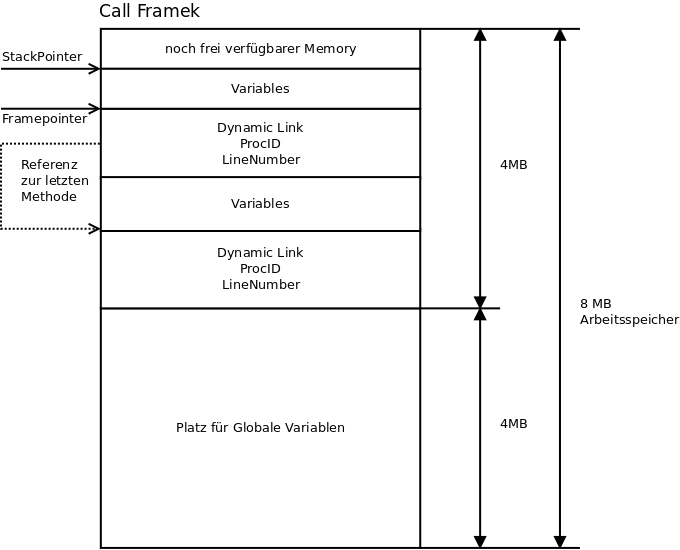
\includegraphics[width=0.9\textwidth]{./media/images/interpreter/memory/stackframe.png}
\label{fig:stackframe1} 
\caption{Aufbau des von uns verwendeten Stack Frames}
\end{center}
\end{figure}
%--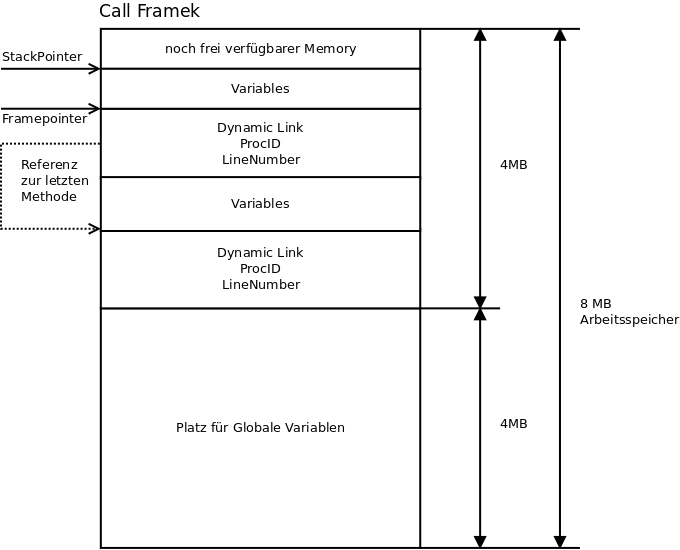
\includegraphics[scale=0.3]{./media/images/interpreter/memory/stackframe.png}

\subsection{Aufbau des Memorys}
Da wir für unser Projekt nicht sehr viel Arbeitsspeicher benötigen, wurden 8 MB Arbeitsspeicher für den Memory reserviert.
Wie man in \ref{fig:stackframe1} erkennen kann, wurde dieser in 2 Hälften geteilt wovon der untere Teil für Globale Variablen und der obere Teil für Methoden verwendet wird.
\newpage

\subsubsection{Anlegen einer neuen Methode}
\begin{enumerate}
 \item Die Zeilennummer wird in den Speicher geschrieben (Größe von 4 Byte)
 \item Der Methoden-Name im Speicher vermerkt (Größe von 4 Byte)
 \item Eine Referenz zur letzten Methode in den Speicher geschrieben (Größe von 4 Byte)
 \item Nun wird der FramePointer auf\footnote{Untere Referenzadresse im Memory} den selben Wert wie der StackPointer\footnote{Obere Referenzadresse im Memory} gesetzt.
 \item Zum StackPointer werden nun die Variablen-Größen hinzugefügt.
\end{enumerate}
 
\subsubsection{Schließen einer Methode}
\begin{enumerate}
 \item Stackpointer wird auf FramePointer gesetzt (Variablen werden entfernt).
 \item 4 Bytes werden vom Stackpointer abgezogen, um nun zur Referenz zu gelangen
 \item Nun können wir den FramePointer aus dem Dynamic Link auslesen und setzten.
 \item Den StackPointer verringern wir nun um den vorherigen Methoden-Namen und um die vorher verwendete Zeilen-Nummer.
\end{enumerate}

Da bei der Speicherverwaltung viele Fehler auftreten könnten ist es wichtig das diese mit verschiedensten Exceptions abgefangen werden.

\subsubsection{Speicherverwaltung}
Die statische Klasse Memory beinhaltet alle Funktionen welche für den Interpreter notwenig sind.

Es werden verschiedene Datentypen unterstützt:
\begin{itemize}
 \item int - 4 Byte
 \item float - 4 Byte
 \item char - 2 Byte 
 \item boolean - 1Byte
 \item string - 4 Byte
\end{itemize}

Hierbei sind die Bytegrößen zu beachten, wobei bei dem Datentyp String nur die String Adresse gespeichert wird. Alle Variablen können
mit der nötigen Adresse und der zum Variablennamen Passenden Funktion Abgefragt werden.

\subsection{Interpreter}
Dadurch, dass wir eine einfache Darstellung der aktuellen Variablen und den Ablauf des Programmes nicht verändern wollten, kam für 
uns nur der Abstrakte Syntax Baum Interpreter in Frage.

Es wurden einige Vorgaben gemacht, um ein zusammenarbeiten zwischen Compiler und Interpreter möglich zu machen. Somit konnten Nodes
nur in einer gewissen Reihenfolge auftreten.
\subsection{Statements}
\subsubsection{Assign}
Bei einem Assign wird eine bestimmte Variable in den Memory geschrieben. Bevor dies jedoch geschehen kann ist es notwendig,
den Datentyp herauszufinden. Dafür wird der Typ des Rechten Knotens geprüft.

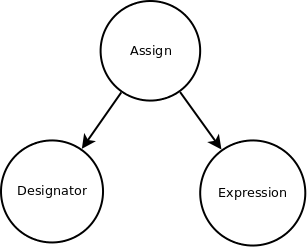
\includegraphics[width=0.4\textwidth]{./media/images/interpreter/syntaxbaum/statements/assign.png}

\subsubsection{Startsequenz}
Mithilfe der Startsequenz, wird durch das ganze Programm durchiteriert.

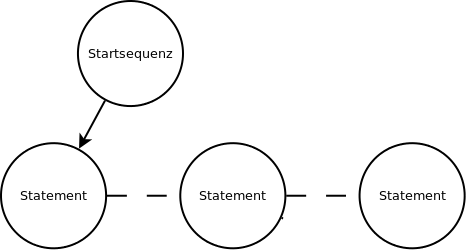
\includegraphics[width=0.4\textwidth]{./media/images/interpreter/syntaxbaum/statements/startsequenz.png}

\subsubsection{Trap}
Die Trap wird dazu benötigt, um einen Unterprogrammaufruf welcher keine Rückgabeparameter besitzt zu beenden.

\subsubsection{If}
Auf der Linken Seite des Knotens stehen die Bedingungen, auf der Rechten Seite steht das zu ausführende Programm, wenn die Bedingung
true ergibt.

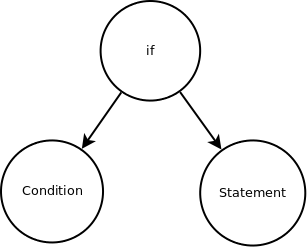
\includegraphics[width=0.4\textwidth]{./media/images/interpreter/syntaxbaum/statements/if.png}

\subsubsection{Ifelse}
Das Ifelse ist grundsätzlich genauso aufgebaut wie das If. Der wesentliche Unterschied besteht darin, dass sobald die Condition
false ergibt, die andere if Funktion abgearbeitet wird.

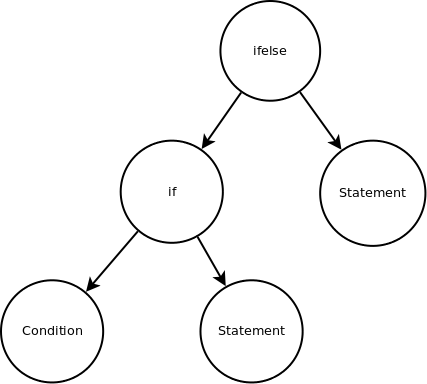
\includegraphics[width=0.4\textwidth]{./media/images/interpreter/syntaxbaum/statements/ifelse.png}

\subsubsection{While}
Funktioniert ähnlich wie ein If, nur das das Statement so lange abgearbeitet wird bis die Condition False ergibt.

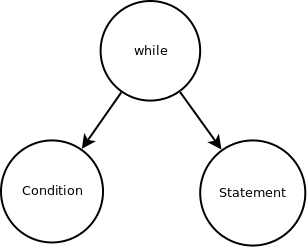
\includegraphics[width=0.4\textwidth]{./media/images/interpreter/syntaxbaum/statements/while.png}

\subsection{Call}
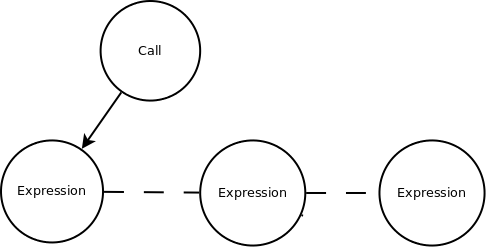
\includegraphics[width=0.4\textwidth]{./media/images/interpreter/syntaxbaum/statements/call.png}

Sobald ein Call aufgerufen wird, wird zuerst anhand des Namens überprüft um welchen Typen von Call es sich handelt.

\subsubsection{print}
Mit diesem Command wird ein Char Zeichen dem StdInOut Interface übergeben. Somit kann dieses danach vom GUI ausgeben werden.

\subsubsection{read}
Wenn Read aufgerufen wird werden vom Interface StdInOut Char Variablen eingelesen und diese als Return Wert gesetzt.

\subsubsection{length}
Hier kann man die Länge eines Strings bestimmen lassen, dieser wird wiederum als Return Wert gesetzt.

\subsubsection{time}
Dient zum Bestimmen der Zeit, welche wiederum als Return Wert zurückgegeben wird.

\subsubsection{Normaler Aufruf}
Sobald ein Aufruf erfolgt, werden alle Variablen welche übergeben werden sollen in einem Objekt zwischengespeichert. Nun kann ein
neues Memory Frame geöffnet werden. Die Variablen, welche in einem Objekt zwischengespeichert wurden, können nun in das neue
Memory Frame übertragen werden.

Nun wird eine Startsequenz ausgeführt, damit der Unterprogrammaufruf abgearbeitet werden kann.

\subsection{Designators}
Auf Designatorn werden bestimmte Werte gespeichert. Weiters sind sie für die richtige Zuweisung der Adresse notwendig.
Hier wird in 3 Grundtypen unterschieden:


\subsubsection{Ident}
Wenn ein Ident aufgerufen wird, werden verschiedene Faktoren geprüft.
\begin{itemize}
 \item Falls der Identifer Global ist, wird der GlobalPointer plus die Objektadresse gerechnet:
 \begin{lstlisting}[language=JAVA]
 adr = Memory.getGlobalPointer() + obj.adr;	
  \end{lstlisting}
  andernfalls wird anstatt des GlobalenPointers der FramePointer des Aktuellen Aufrufes verwendet.
   \begin{lstlisting}[language=JAVA]
 adr = Memory.getFramePointer() + obj.adr;
  \end{lstlisting}
 \item Wenn der Identifer eine Referenz auf eine Adresse ist, wird hier die gespeicherte Adresse geladen.
\end{itemize}



\subsubsection{Dot}
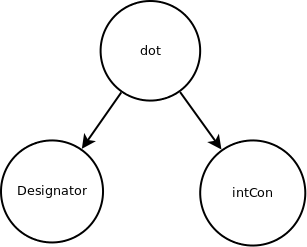
\includegraphics[width=0.4\textwidth]{./media/images/interpreter/syntaxbaum/designators/dot.png}

Wird für Strukturen angewant. Um die richtige Adresse für eine Variable in der Struktur zu bekommen muss die Adresse des Linken
Knotens mit der Rechten Seite des Knotens addiert werden.

\begin{lstlisting}[language=JAVA]
return Adr(p.left) + p.right.val
\end{lstlisting}

\subsubsection{Index}
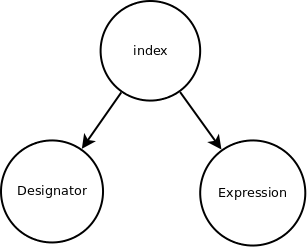
\includegraphics[width=0.4\textwidth]{./media/images/interpreter/syntaxbaum/designators/index.png}

Um den Index auszurechnen ist es notwendig die Expression auf der rechten Seite aufzulösen.
Nun kann die Adresse berechnet werden. Diese setzt sich aus der Adresse der rechten Seite und der Größe der Elemente mal dem 
verwendeten Index zusammen.

\begin{lstlisting}[language=JAVA]
return Adr(p.left) + p.left.type.elemType.size * index;
\end{lstlisting}

\subsection{Expressions}
Expressions werden grundsätzlich für Berechnungen und Typconvertierungen verwendet, aus diesem Grund ist es wichtig dass jeder Datentyp seine
eigene Expressions Methode besitzt.

\subsection{Conditions}
Conditions werden zur Verwendung von if-Bedingungen und für Schleifen benötigt.

%	--------------------------------------------------------
% 	Kalkulation
%	--------------------------------------------------------
\section{Kalkulation}


%	--------------------------------------------------------
% 	Arbeitseinteilung
%	--------------------------------------------------------
\section{Arbeitseinteilung}